\section{Imperfect plate and spheres}
\label{sec:3:imperfect-plates}

Python numerical approach, gaussian modes (vibration modes of a spherical plane), perlin noise

\begin{figure}[!htbp]
  \centering
  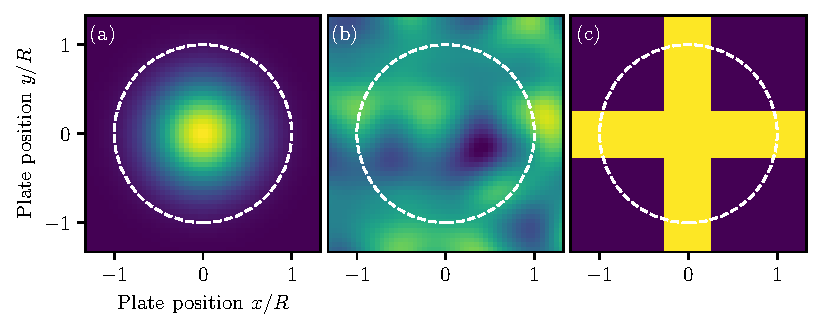
\includegraphics[width=\textwidth]{../figures/imperfect-plates.pdf}
  \caption{A selection of imperfect plates. \textbf{(a)} A simple gaussian displacement in the same size as the sphere. \textbf{(b)} Random excitations in the shape of \textit{perlin noise}. \textbf{(c)} a cross-shape in the center of the plate. All displacements are in the size of $0.1R$.}
  \label{fig:3:imperfect-plates}
\end{figure}

% \begin{figure}[!htbp]
%   \centering
%   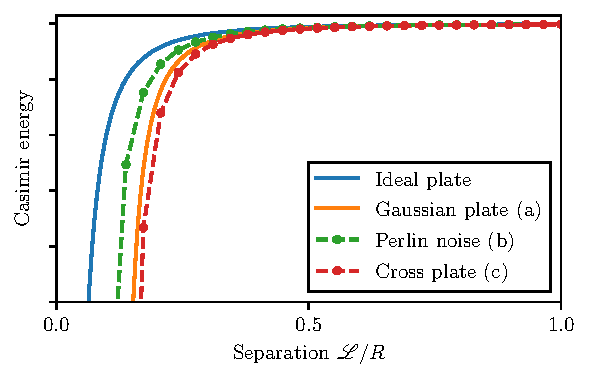
\includegraphics[width=0.7\textwidth]{../figures/casimir-potential-imperfect-plates.pdf}
%   \caption{Casimir potential in the PFA for the different noisy plates displayed in \cref{fig:3:imperfect-plates}. It becomes evident, that local deviations in the distance between the plate and the sphere in the order of $\Delta \mathscr{L} \sim 0.1R$ only contribute a small factor to the form of the potential.}
%   \label{fig:3:casimir-imperfect-plates}
% \end{figure}
\begin{figure}[!htbp]
  \centering
  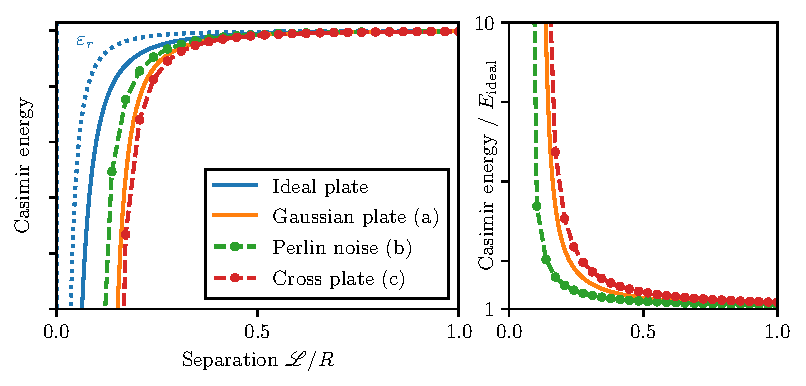
\includegraphics[width=\textwidth]{../figures/casimir-potential-imperfect-plates-relative.pdf}
  \caption{Casimir energy for the different noisy plates displayed in \cref{fig:3:imperfect-plates}. It becomes evident, that local deviations in the distance between the plate and the sphere in the order of $\Delta \mathscr{L} \sim 0.1R$ increase the Casimir force exponentially for very small separations. Larger separations however are seemingly unaffected.}
  \label{fig:3:casimir-imperfect-plates}
\end{figure}